\subsection{利用期限结构模型进行套利定价}

这一节主要介绍利率二叉树，以及使用利率二叉树给债券等衍生品进行定价。


\subsubsection{基本概念}


1. 基本概念

\begin{itemize}
\item 假设: A binomial model is a model that assumes that interest rate can take only one of two possible values in the next period， an upper path (U) and a lower path (L). 【利率未来有两个可能:upper path (U)和 lower path (L)。】
\end{itemize}

\begin{itemize}
\item The interest rates at each node are one-period forward rates corresponding to the nodal period.
\end{itemize}

在利率二叉树中，第一个利率 \({\mathrm{i}}_{0}\) 是 spot rate，通常是已知的；之后的利

率，比如 \({\mathrm{i}}_{1，\mathrm{U}}\text{ 、 }{\mathrm{i}}_{1，\mathrm{L}}\text{ 、 }{\mathrm{i}}_{2，\mathrm{{UU}}}\text{ 、 }{\mathrm{i}}_{2，\mathrm{{LL}}}\text{ 、 }{\mathrm{i}}_{2，\mathrm{{LU}}}\) 等，是 forward rate。

\begin{center}
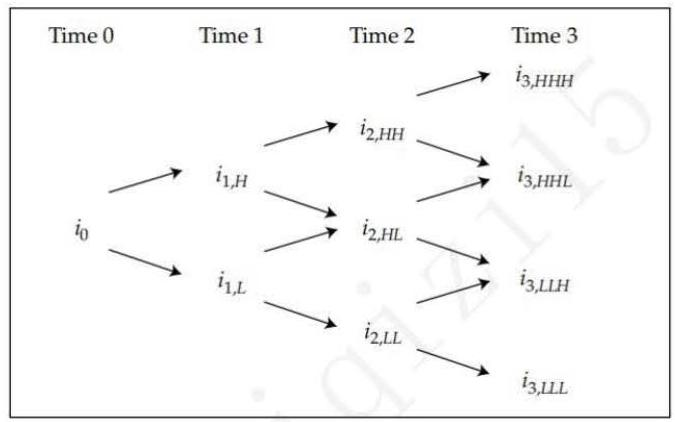
\includegraphics[width=0.5\textwidth]{images/01963dfb-ec81-7114-affc-d6d56ed48aa5_39_485_798_675_422_0.jpg}
\end{center}
\hspace*{3em} 



\subsubsection{利率二叉树求债券价格}


2. 利率二叉树求债券价格

\begin{itemize}
\item 二叉树的构建， 是由前往后的过程。【关于二叉树的构建， 不是本节的重点， 将会在 The Art of Term Structure Models 章节介绍】
\end{itemize}

\begin{itemize}
\item 求债券或其他金融产品价格， 是由后往前的过程 Backward induction valuation。
\end{itemize}

\begin{itemize}
\item Backward induction valuation: Valuing bond by moving backward from last period to time zero.
\end{itemize}

\begin{itemize}
\item 过程: Bond value at any node:
\end{itemize}

Average PV of two possible values from next period;

 Discount rate is the one-period forward rate at that node.

\begin{itemize}
\item 【一般利率二叉树的步数比债券价格二叉树少一步】
\end{itemize}

Example 1:【利用利率二叉树求债券价格】

\begin{itemize}
\item Assume that the six-month spot rates is 5\% respectively. The six-month rate in six months will be either 4.50 or 5.50 with equal probability. Calculate the expected discounted value of a one-year zero coupon bond with par value of \$1000.
\end{itemize}

\begin{center}
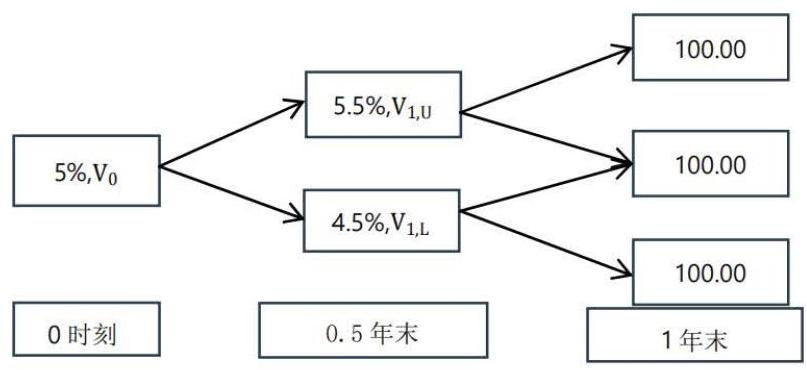
\includegraphics[width=0.6\textwidth]{images/01963dfb-ec81-7114-affc-d6d56ed48aa5_40_238_265_807_370_0.jpg}
\end{center}
\hspace*{3em} 

\begin{itemize}
\item 计算过程:
\end{itemize}

 首先，计算最后节点债券价格。

 其次，求期望，再贴现。

\[
{\mathrm{V}}_{1，\mathrm{U}} = \frac{1000}{1 + {5.5}\% /2} = {973.236}
\]

\[
{\mathrm{V}}_{1，\mathrm{\;L}} = \frac{1000}{1 + {4.5}\% /2} = {977.9951}
\]

\[
{\mathrm{V}}_{0} = \frac{\left( {973.236} \times  {50}\%  + {977.9951} \times  {50}\% \right) }{1 + 5\% /2} = {951.82}
\]

 此债券的 expected discounted value 是 951.82.

【切记:勿忘票面利息(如有)，折现时要体现出来。另外， 利率二叉树中的两个可能是等概率的】

\begin{itemize}
\item 使用下面的利率二叉树， 计算债券价格。债券基本信息: 到期时间 3 年， coupon 按年支付， coupon rate 是 5\%， 票面价值是 100 .
\end{itemize}

\begin{center}
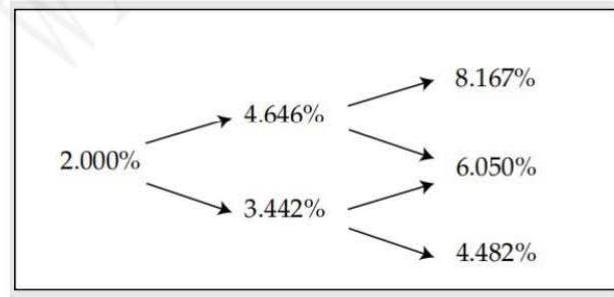
\includegraphics[width=0.5\textwidth]{images/01963dfb-ec81-7114-affc-d6d56ed48aa5_40_511_1416_614_297_0.jpg}
\end{center}
\hspace*{3em} 

\begin{itemize}
\item 计算过程:
\end{itemize}

✓ 首先，计算最后节点债券价格。

\[
{\mathrm{V}}_{2，\mathrm{{UU}}} = \frac{{100} + 5}{1 + {8.167}\% } = {97.0721}
\]

\[
{\mathrm{V}}_{2，\mathrm{{UL}}} = \frac{{100} + 5}{1 + {6.050}\% } = {99.0099}
\]

\[
{\mathrm{V}}_{2，\mathrm{{LL}}} = \frac{{100} + 5}{1 + {4.482}\% } = {100.4958}
\]

\begin{center}
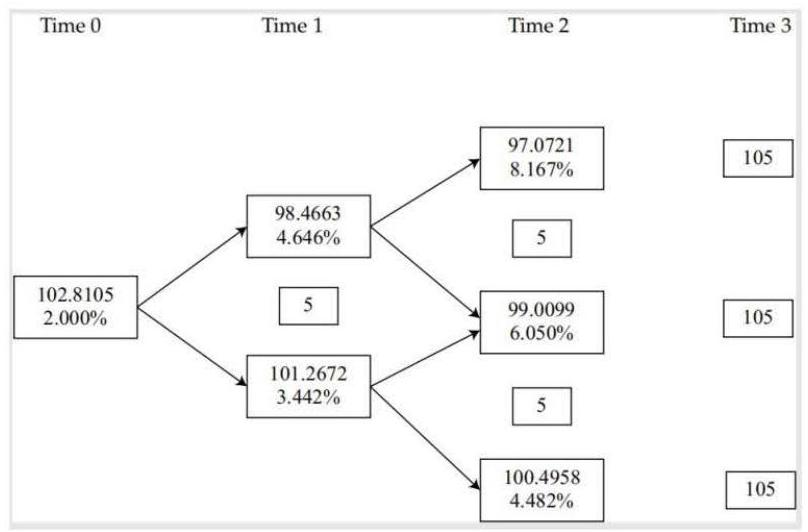
\includegraphics[width=0.6\textwidth]{images/01963dfb-ec81-7114-affc-d6d56ed48aa5_41_421_214_808_532_0.jpg}
\end{center}
\hspace*{3em} 

✓其次，最后节点的 PV，求期望。期望价格加上 coupon 再贴现到前一时刻。不断重复这一步骤， 直到贴现到 0 时刻。

\[
{\mathrm{V}}_{1，\mathrm{U}} = \frac{\left( {{97.0721} \times  {50}\%  + {99.0099} \times  {50}\% }\right)  + 5}{1 + {4.646}\% } = {98.4663}
\]

\[
{\mathrm{V}}_{1，\mathrm{\;L}} = \frac{\left( {{99.0099} \times  {50}\%  + {100.4958} \times  {50}\% }\right)  + 5}{1 + {3.442}\% } = {101.2672}
\]

\[
{\mathrm{V}}_{0} = \frac{\left( {{98.4663} \times  {50}\%  + {101.2672} \times  {50}\% }\right)  + 5}{1 + 2\% } = {102.8105}
\]

 此债券的价格是 102.8105.

\begin{itemize}
\item 事实上， 使用等概率 (上升/下降) 利率二叉树计算出的债券价格和债券的市场价格未必相同。
\end{itemize}

This is because the 0.5 probabilities are the assumed true probabilities of price movements.

\begin{itemize}
\item 可以通过调整利率二叉树的利率或者利率二叉树中的概率(这里概率叫作 risk-neutral probabilities) 使得 expected discounted value 等于市场价格。
\end{itemize}

\begin{itemize}
\item Any difference between the risk-neutral and true probabilities is referred to as the interest rate drift.
\end{itemize}


\subsubsection{利率二叉树求期权价格}


3. 利率二叉树计算期权价格

\begin{itemize}
\item What is the price of a call option， maturing in six months， to purchase \(\$ 1，{000}\) face value of a then six-month zero at \$975? Assuming six-month and one-year spot rates are 5\% and 5.15\% respectively.
\end{itemize}

The interest rate tree:

\begin{center}
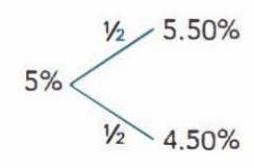
\includegraphics[width=0.2\textwidth]{images/01963dfb-ec81-7114-affc-d6d56ed48aa5_42_698_232_254_168_0.jpg}
\end{center}
\hspace*{3em} 

✓ 计算: Call 的 payoff

\begin{center}
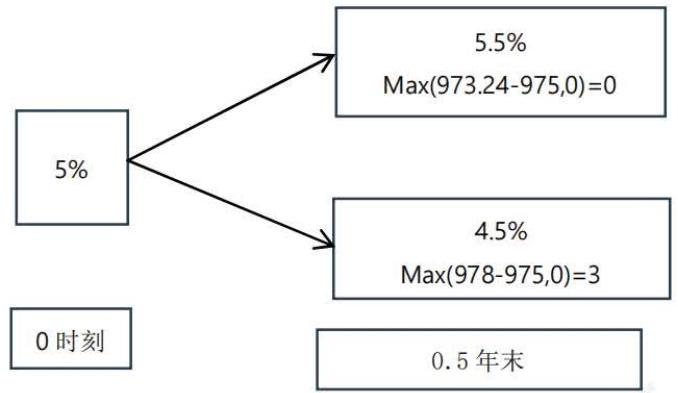
\includegraphics[width=0.5\textwidth]{images/01963dfb-ec81-7114-affc-d6d56ed48aa5_42_424_471_678_393_0.jpg}
\end{center}
\hspace*{3em} 

\begin{itemize}
\item The expected discounted value of option \(= \frac{\left( 0 \times  {50}\%  + 3 \times  {50}\% \right) }{1 + 5\% /2} = {1.46}\)
\end{itemize}

\subsubsection{定期国债互换}


4. Constant Maturity Treasury Swap

\begin{itemize}
\item The rate tree can be used to price a constant-maturity Treasury (CMT) swap. In the example， the strike (fixed rate) is 5.0\% such that the swap pays: \({1000000} \times  \frac{{y}_{\mathrm{{CMT}}} - 5\% }{2}\) every six months until it matures， where \({y}_{\mathrm{{CMT}}}\) is a semiannually compounded yield， of a p redetermined maturity， on the payment date. 风险中性概率及利率二叉树如下， 求 CMT swap 的价格。
\end{itemize}

\begin{center}
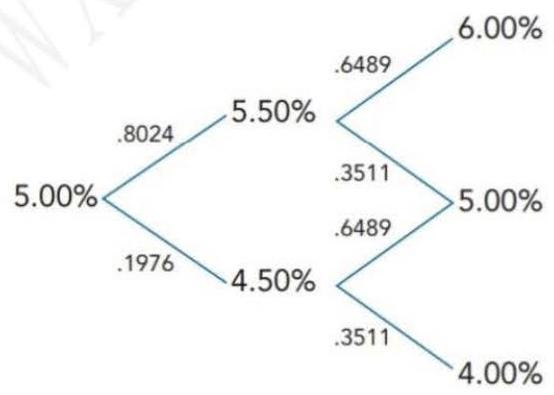
\includegraphics[width=0.4\textwidth]{images/01963dfb-ec81-7114-affc-d6d56ed48aa5_42_537_1395_554_395_0.jpg}
\end{center}
\hspace*{3em} 

 计算: 在 1 年末互换的收益

\[
\frac{6\%  - 5\% }{2} \times  1，{000}，{000} = {5000}
\]

\[
\frac{5\%  - 5\% }{2} \times  1，{000}，{000} = 0
\]

\[
\frac{4\%  - 5\% }{2} \times  1，{000}，{000} =  - {5000}
\]

在 6 个月末收益，再加上 1 年末收益期望的现值。

\[
\frac{{5.5}\%  - 5\% }{2} \times  1，{000}，{000} + \frac{{5000} \times  {0.6489} + 0 \times  {0.3511}}{1 + \frac{{5.5}\% }{2}} = {2500} + {3157.66}
\]

\[
= {5657.66}
\]

\[
\frac{{4.5}\%  - 5\% }{2} \times  1，{000}，{000} + \frac{0 \times  {0.6489} + \left( {-{5000}}\right)  \times  {0.3511}}{1 + \frac{{4.5}\% }{2}}
\]

\[
=  - {2500} - {1716.87} =  - {4216.87}
\]

未来现金流期望的现值，求出当前的收益。

\[
\frac{{5657.66} \times  {0.8024} + \left( {-{4216.87}}\right)  \times  {0.1976}}{1 + \frac{5\% }{2}} = {3616.05}
\]

所以， 1 年期的 CMT 互换的价格是 3616.05. 5. 其他

\begin{center}
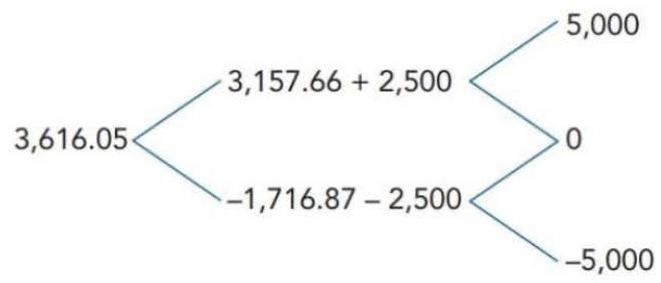
\includegraphics[width=0.5\textwidth]{images/01963dfb-ec81-7114-affc-d6d56ed48aa5_43_487_207_661_283_0.jpg}
\end{center}
\hspace*{3em} 

\begin{itemize}
\item OAS
\end{itemize}

\begin{itemize}
\item Option-adjusted spread (OAS) is a widely-used measure of the relative value of a security， that is， of its market price relative to its model value.
\end{itemize}

\begin{itemize}
\item OAS is defined as the spread such that the market price of a security equals its model price when discounted values are computed at risk-neutral rates plus that spread. 【OAS 是一种 spread， 在构造含权债的利率二叉树时， 有时会对 spread 进行调整， 让其折现价格=市场价格。】
\end{itemize}

\begin{itemize}
\item BSM model 不能给债券期权定价:
\end{itemize}

\begin{itemize}
\item the model assumes that the price of stock follows a random process， but bond price must converge to its face value at maturity. [BSM 假设标的资产价格是 random，而债券价格最终会趋向面值，并不是随机的。】
\end{itemize}

\begin{itemize}
\item the model assumes that the volatility of stock price is constant， but the volatility of bond price must eventually get smaller as the bond approaches maturity. 【BSM 假设标的资产价格的波动率是恒定的， 但是债券价格的波动率会慢慢趋向于 0 】
\end{itemize}

\begin{itemize}
\item the model assumes the short-term interest rate is constant， but this assumption obviously does not work for pricing analysis of bond option. 【BSM 假设 short-term interest rate 是恒定的， 但是这对于债券而言是不合适的。】
\end{itemize}

\begin{itemize}
\item Recombining tree vs. non-recombining tree
\end{itemize}

\begin{itemize}
\item The non-recombining trees have economic reasonableness， but are difficult or even impossible to implement.
\end{itemize}

After \(\mathrm{N}\) periods， there are \({2}^{\mathrm{N}}\) possible states for non-recombining trees.

After \(\mathrm{N}\) periods， there are \(\mathrm{N} + 1\) possible states for recombining trees. 【大部分利率二叉树是这样】

\begin{center}
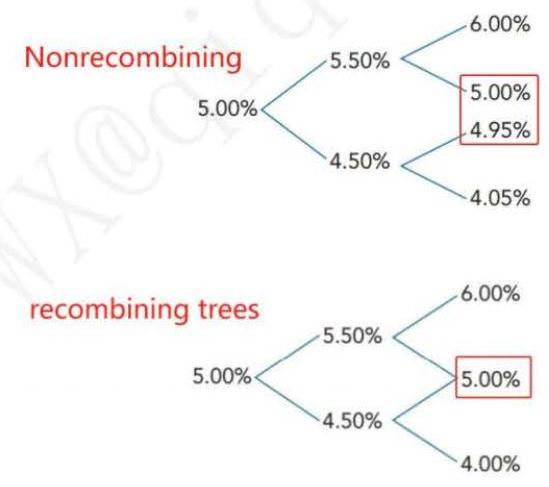
\includegraphics[width=0.4\textwidth]{images/01963dfb-ec81-7114-affc-d6d56ed48aa5_44_552_1178_549_487_0.jpg}
\end{center}
\hspace*{3em} 


\subsubsection{其他}


\subsection{预期、风险溢价、凸性与
期限结构(☆☆)}



\begin{itemize}
\item 简介: 这一节原版书通过利率二叉树或者 spot rate 与债券价格的关系， 来说明下面这个问题:
\end{itemize}

 从 3 个角度解释， 为什么利率期限结构是 flat， upward-sloping， 或 downward-sloping.

Expectations of future short-term rates

Volatility of short-term rates

Interest rate risk premium

\subsubsection{预期}

(1) Expectations of future short-term rates。

\begin{itemize}
\item 根据一级的纯预期理论， 如果预期未来的利率 (forward) 上升/不变/下降， 那么利率期限结构是 upward-sloping/flat/downward-sloping.
\end{itemize}

但在实际中， 短期预期会因政策变化而变化


补充: Pure Expectations Theory 纯预期理论

\hspace*{1em} - 假设: 投资者是 risk neutrality (risk-free rate)

\hspace*{1em} - It says that the forward rate is an unbiased predictor of the

\hspace*{2em} future spot rate 【远期利率是对未来的即期利率的无偏估

\hspace*{2em} 计。】

\hspace*{1em} - 结论: 长期债券的收益率是由市场参与者对未来利率的预

\hspace*{2em} 期值所决定的。换句话说， 市场预期未来利率(forward rate)

\hspace*{2em} 上升， 长期收益率曲线会向上倾斜; 如果市场预期未来利

\hspace*{2em} 率(forward rate)下降，长期收益率曲线会向下倾斜。










\subsubsection{波动性与凸性}

(2) Volatility of short-term rates

\begin{itemize}
\item 在利率期限结构是 flat 这一设定下，因为利率存在波动性， 会使得利率期限结构向下倾斜。
\end{itemize}

\begin{itemize}
\item 利率的波动性， 用利率二叉树体现。
\end{itemize}

9 原因:债券价格曲线是具有凸性的。

\begin{itemize}
\item This convexity effect arises from the mathematical fact， a special case of Jensen's Inequality 詹森不等式:
\end{itemize}

\begin{center}
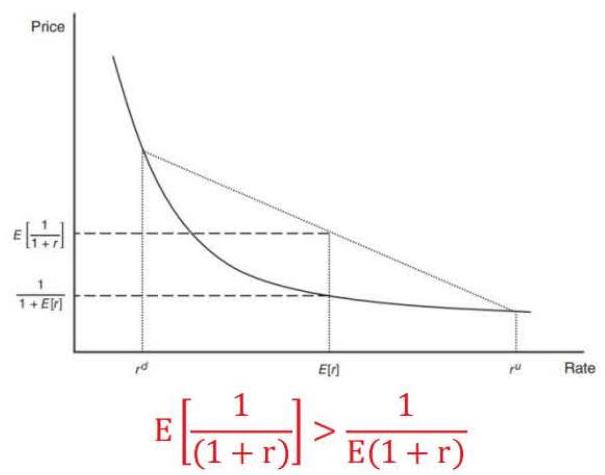
\includegraphics[width=0.5\textwidth]{images/01963dfb-ec81-7114-affc-d6d56ed48aa5_46_517_206_605_475_0.jpg}
\end{center}
\hspace*{3em} 

 Introducing volatility， yield is reduced by convexity.




\subsubsection{Bond Return Components 债券收益拆分}


(3) Bond Return Components 债券收益拆分

\begin{itemize}
\item 可以分解为三个部分:
\end{itemize}

 时间推移带来的收益 (由远期利率 forward rate 决定)。

 利率变化带来的收益 (与久期 duration 成反比)。

 波动性带来的收益 (与凸性 convexity 成正比)。

\begin{itemize}
\item Risk-averse investors will require compensation (即 Risk premium)for bearing interest rate risk.
\end{itemize}

\(\rangle\) 前面我们在讨论利率二叉树，通常假设是投资者风险中性的。这里考虑的投资者是风险厌恶的(Risk-averse investors)。

\begin{itemize}
\item 风险厌恶投资者要求债券的预期回报率高于短期利率，并与利率风险成比例。
\end{itemize}

 Risk averse investors demand higher expected returns for bonds with greater interest rate risk.

 The interest rate risk of a bond over the next instant may be measured by its duration with respect to the interest rate factor， and that risk-averse investors demand a risk premium proportional to duration.

This risk premium may depend on time and on the level of rates， but not on the characteristics of any individual bond. 【风险溢价取决于时间和利率水平， 但与单个债券自身的特性无关。】

The risk premium were constant and denoted by \(\lambda\) .

\begin{itemize}
\item The expected return equation for risk-averse investors :
\end{itemize}

\[
\mathrm{E}\left( \frac{\mathrm{{dP}}}{\mathrm{P}}\right)  = {\mathrm{r}}_{0}\mathrm{{dt}} + \lambda \mathrm{{Ddt}}
\]

 \(\mathrm{E}\left( \frac{\mathrm{{dP}}}{\mathrm{P}}\right)\) :债券的预期回报率。其中， \(\mathrm{{dP}}\) 是债券价格的微小变化， \(\mathrm{P}\) 是债券的初始价格

 \({\mathrm{r}}_{0}\) : 短期利率

 dt: 一个微小的时间间隔

 \({\mathrm{r}}_{0}\mathrm{{dt}}\) : 因时间推移而产生的回报。

 λ: 风险溢价

 D: 债券的久期

 λDdt:表示因利率风险而产生的额外回报。久期衡量了债券价格对利率变动的敏感性， 风险溢价反映了投资者因承担这种利率风险而要求的额外补偿。

\begin{itemize}
\item For example， that the short-term rate is 1\%， that the duration of a bond is five， and that the risk premium is 10 basis points per year of duration risk.
\end{itemize}

 The bond’s expected return \(= 1\%  + 5 \times  {0.1}\%  = {1.5}\%\) per year.


\subsection{利率期限结构模型的方法：漂移}

\subsection{利率期限结构模型的方法：波动率和分布}




这两个 chapter 内容整理到了一起

本节主要介绍利率二叉树的构建，同时假设利率上升和下降的概率相等。在这些模型中，通常将利率的变化分为两个部分：漂移项（drift，也叫趋势项）和波动项（volatility）。

\begin{itemize}
\item The Art of Term Structure Models: Drift
    \begin{itemize}
    \item Model 1: no drift
    \item Model 2: constant drift
    \item Model 3: time-dependent drift
    \item Model 4: mean-reverting drift
    \end{itemize}

\item Volatility and Distribution
    \begin{itemize}
    \item Time-dependent volatility
    \item Model 3: 
    \item Volatility as a function of the short rate
        \begin{itemize}
        \item The Cox-Ingersoll-Ross (CIR) model
        \item Lognormal model (model 4)
        \item Lognormal model with deterministic drift
        \item Lognormal model with mean reversion
        \end{itemize}
    \end{itemize}
\end{itemize}



\subsubsection{    \textbf{模型一(Distribution of short rates after one year， Model 1)}}



    \begin{itemize}
    \item The continuously compounded， instantaneous rate \( r \) is assumed to evolve according to the following equation:
            \[
            dr = \sigma dw
            \]
            \[
            dw = \epsilon dt
            \]
        \begin{itemize}
        \item \( dr \): change in interest rates over \( dt \).
        \item \( dt \): a small time interval， measured in years.
        \item \( \sigma \): annual basis-point volatility of rate changes.
        \item \( dw \): normally distributed random variable with \( N(0， \sqrt{dt}) \).
        \item \( \epsilon \) 是随机变量；\( \epsilon \) 认为未来利率只有两种可能，即只有两种可能。大多数情况下简化，取值为“−1”或“+1”。
        \end{itemize}
    \item Expected change of the rate: \( E(dr) = 0 \).
    \item Standard deviation of the rate: \( \text{Std.}(r) = \sigma \sqrt{dt} \).
    \item 第一期利率是 \( r_0 \)，第二期利率是 \( r_0 + dr \)，即 \( r_0 + \sigma \sqrt{dt} \times \epsilon \)（\(\epsilon\) 取值为“−1”或“+1”）。未来利率是 \( r_0 + \sigma \sqrt{dt} \) 或者 \( r_0 - \sigma \sqrt{dt} \)，可得利率二叉树：
        \begin{center}
        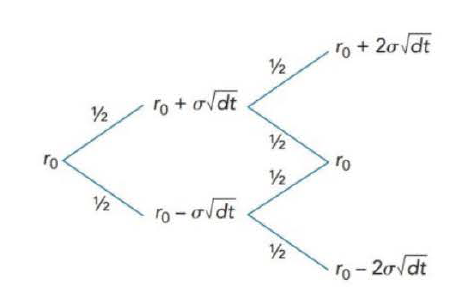
\includegraphics[width=0.8\textwidth]{images/twotree.png}
        \end{center}
    \item 例子：the current value of the short-term rate is 6.18\%， that volatility equals 113 basis points per year， and the time interval under consideration is one month or \( \frac{1}{12} \) years.
    \item 
                    \[
                    dr = \sigma dw = \sigma \sqrt{dt}
                    \]
                    \[
                    dr = 11.3\% \times \sqrt{\frac{1}{12}} = 0.326\%
                    \]
    \item 计算：
                    \begin{align*}
                    6.18\% + 0.326\% &= 6.506\% \\
                    6.18\% - 0.326\% &= 5.854\% \\
                    6.506\% + 0.326\% &= 6.832\% \\
                    5.854\% - 0.326\% &= 5.528\%
                    \end{align*}
    
        \begin{center}
                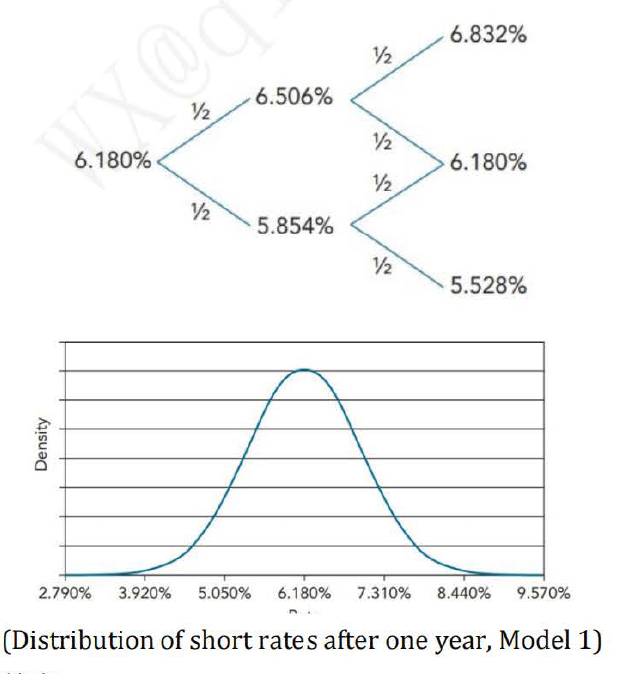
\includegraphics[width=0.8\textwidth]{images/model1.png}
        \end{center}
    \item Model 1 的缺点：            
        \begin{itemize}
        \item The no-drift assumption does not give enough flexibility to accurately model basic term structure shapes. The result is a downward-sloping predicted term structure due to a larger convexity effect. 【容易出现负利率】
            \begin{itemize}
                \item \textbf{处理方法：}
                    \begin{itemize}
                \item 改变利率的分布，可以假设为非正态分布。
                \item 如果出现负的利率，令这个负的利率等于 0。
                    \end{itemize}

            \end{itemize}
        \item Model 1 predicts a flat term structure of volatility， whereas the observed volatility term structure is hump-shaped， rising and then falling.
        \item Model 1 \textcolor{red}{only has one factor， the short-term rate}. Other models that incorporate additional factors (e.g.， drift， time-dependent volatility) form a richer set of predictions.
        \item Model 1 implies that any change in the short-term rate would lead to a parallel shift in the yield curve. 【收益率曲线的平行移动不符合现实】
        \end{itemize}
    \end{itemize}
    




\subsubsection{Model 2: Drift and risk premium 模型二}


\begin{itemize}
    \item MODEL 2 adds a drift to Model 1， in order to obtain a richer model in an economically coherent way.
    \[
    dr = \lambda dt + \sigma dw
    \]
    \(\lambda\): annual drift in interest rates.
    \begin{itemize}
        \item Expected change of the rate: \( E(dr) = r \).
        \item Standard deviation of the rate: \( \text{Std.}(r) = \sigma \sqrt{dt} \).
        \item The drift (\(\lambda dt\)) in the risk-neutral process is a combination of the true expected change in the interest rate and of a risk premium.
    \end{itemize}
\end{itemize}

\textbf{利率二叉树：}



\begin{center}
    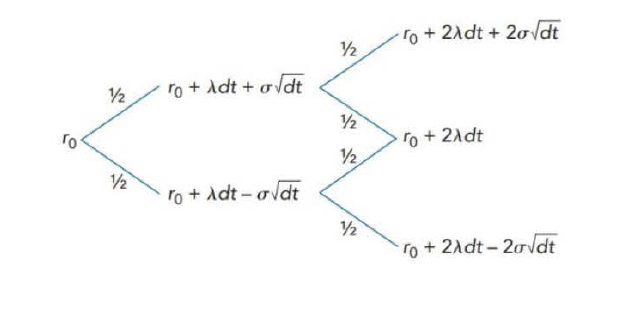
\includegraphics[width=0.8\textwidth]{images/twotree2.png}
    \end{center}

\begin{itemize}
    \item 优点：
    \begin{itemize}
        \item Model 2 is more effective than Model 1.
    \end{itemize}
\end{itemize}

\begin{itemize}
    \item 缺点：
    \begin{itemize}
        \item Model 2 is still not flexible enough because of constant drift.
        \item Model 2 still implies a parallel shift of the term structure curve if the interest rate changes.
    \end{itemize}
\end{itemize}

\subsubsection{Ho-Lee Model:Time-dependent drift}


\begin{itemize}
    \item A drift that varies with time is called a time-dependent drift. 【漂移项随时间变化】
    \item 和 Model 2 一样，the time-dependent drift over each time period represents some combination of the risk premium and of expected changes in the short-term rate.
    \[
    dr = \lambda_1 dt + \sigma dw
    \]
    \(\lambda_t\): a time-dependent drift term.
    \begin{itemize}
        \item It is clear that if \( \lambda_1 = \lambda_2 \) then the Ho-Lee model reduces to Model 2. Also， it should not be surprising that \( \lambda_1 \) and \( \lambda_2 \) are estimated from observed market prices.
    \end{itemize}
\end{itemize}

\textbf{利率二叉树：}
\begin{center}
    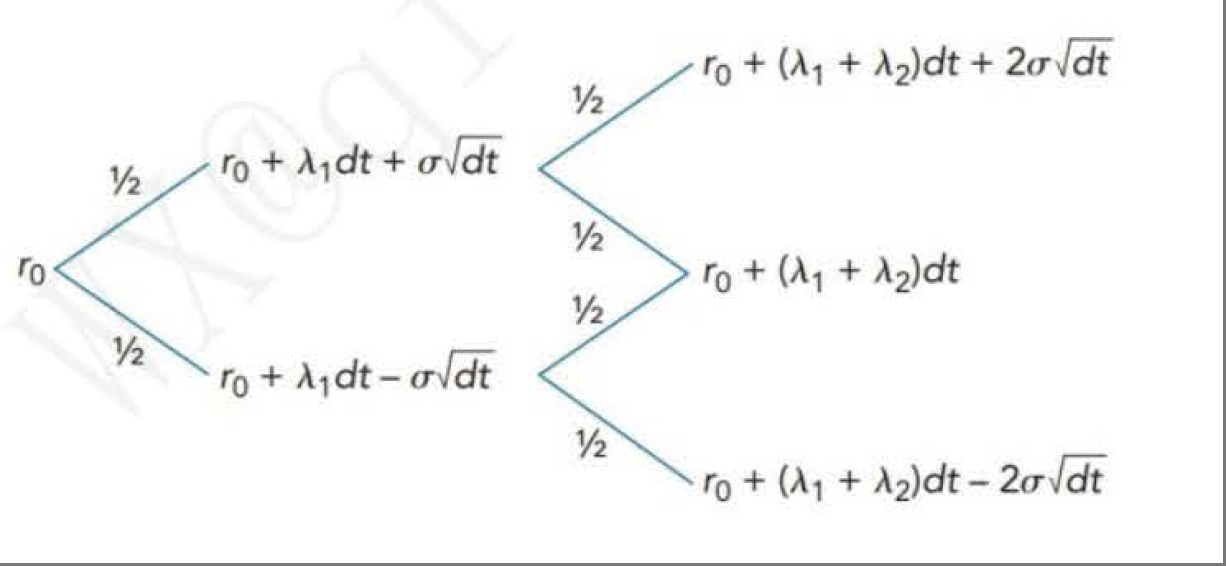
\includegraphics[width=0.8\textwidth]{images/modelHL.png}
    \end{center}
\textbf{Arbitrage-free models 无套利模型：}

    \begin{itemize}
        \item This model assumes bonds trading in the market are correctly priced (arbitrage free).
        \item 无套利模型：确保不存在套利机会来建立模型。通常使用市场上的实际数据和价格来推断当前的期限结构。
        \item For example， an arbitrage-free tree is constructed to properly price on-the-run Treasury securities (i.e.， the model price must match the market price). Then， the arbitrage-free tree is used to predict off-the-run Treasury securities and is compared to market prices to determine if the bonds are properly valued. 【利用 properly price 构建利率二叉树，然后用这个二叉树给一些流动性或其他方面缺乏的金融产品定价】
    \end{itemize}

\begin{itemize}
    \item Need more variables
    \item Models 1 and 2 would be called equilibrium models because no effort has been made to match the initial term structure closely.
    \item 无套利模型通常用于流动性较差或定价不准确的证券价格。
    \item 无套利模型的缺点：
    \begin{itemize}
        \item First， calibrating to market prices is still subject to the suitability of the original pricing model.
        \item Second， 无套利模型假设基础价格是准确的。
    \end{itemize}
\end{itemize}

\textbf{Equilibrium models 均衡模型：}
\begin{itemize}
    \item Describe the dynamics of the term structure using fundamental economic variables that are assumed to affect interest rates. 【希望通过考察影响利率的基本经济因素，来理解不同期限的利率之间的关系】
    \item Ho-Lee Model are Arbitrage-free models.
    \item 如果模型的目的是进行相关分析（即将一个证券与另一个进行比较），通常会使用均衡模型而不是无套利模型。
    \item 实际上，无套利模型和均衡模型之间可能存在明确的界限，可以根据具体情况而定。
\end{itemize}


\subsubsection{Vasicek Model:Mean reversion}


\begin{itemize}
\item 假设经济走向于某种均衡状态 (such fundamental factors as the productivity of capital， long-term monetary policy， and so on)，那么短期利率将呈现均值回归。
    \begin{itemize}
    \item 均值回归是利率的一个重要特征，这与股价价格不同。利率不能无限上升，当利率非常高时，会妨碍经济活动，利率会被调整，最终导致利率下降。另一方面，除了极少数历史例外，名义利率是非负的。因此，短期利率往往存在于预期范围内的波动，并表现出回归到长期利率的趋势。
    \end{itemize}
\item Vasicek model captures mean reversion:
    \[
    dr = \kappa(\theta - r)dt + \sigma dw
    \]
    \(\kappa\): the speed of mean reversion.
    \begin{itemize}
    \item \( \theta \): the long-run mean reversion level.
    \item \( r \): current interest rate level.
    \item Drift term (趋势项): \( \kappa(\theta - r)dt \). The drift combines both interest rate expectations and risk premium.
    \item Stochastic term (随机项): \( \sigma dz \).
        \begin{itemize}
            \item 也叫shock 冲击。表示对短期利率r 的产生的突然的、意外的影响或扰动。
        \end{itemize}
    \end{itemize}
\item When the short-term rate is above its long-run equilibrium value， the drift is negative， driving the rate down toward this long-run value.
\item When the rate is below its equilibrium value， the drift is positive， driving the rate up toward this value.
\item The Vasicek model is not recombining. The tree can be approximated as recombining by averaging the unequal two nodes and recalibrating the associated probabilities (i.e.， no longer using 50\% probabilities for the up and down moves).
    \begin{center}
    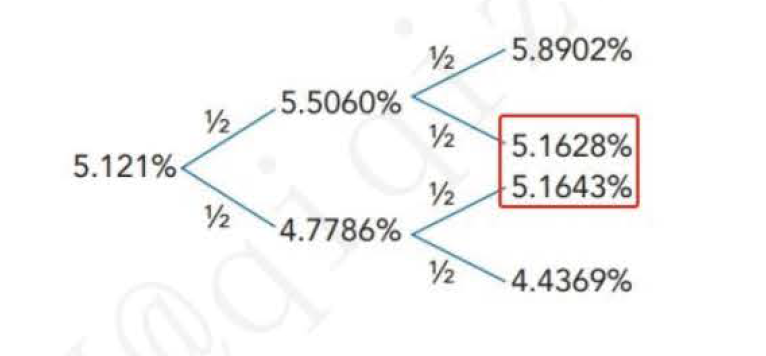
\includegraphics[width=0.8\textwidth]{images/VMODEL.png}
    \end{center}



 \item Vasicek Model: Half Life
    \begin{itemize}
    \item The expectation of the rate in the Vasicek model after \( T \) years is:
        \[
        E(r_T) = r_0 e^{-\kappa T} + \theta \left(1 - e^{-\kappa T}\right)
        \]
    \item The mean-reverting parameter \( k \) is not an intuitive way of describing how long it takes to revert to its long-term goal.
    \item A more intuitive quantity is the factor's half-life \( t \):
        \[
        t = \frac{\ln 2}{\kappa}
        \]
        \begin{itemize}
        \item 半衰期： The time it takes the factor to progress half the distance
         toward its goal.
        \item 例如 \( k = 0.0165 \)，则 \( t = -\frac{\ln 2}{0.0165} \approx 42 \) 年。这意味着短期利率受到冲击后，其影响会长期存在，预期利率需要很久才能从当前值恢复到长期值。
        \item Equivalently， the expected rate takes a very long time to revert from the current rate to \( \theta \). 【简单来说，利率一旦被干扰，要恢复正常要等好久。】
        \end{itemize}
    \item A larger mean reversion adjustment parameter \( k \) will result in a shorter half-life.
    \end{itemize}

    
\item Vasicek Model: Effectiveness
    
    \begin{itemize}
    \item For models without mean reversion， the standard deviation of the terminal distribution after \( T \) years increases with the square root of time. 【在没有均值回归的情况下，随着时间的推移，波动性会增加。】
    \item For the Vasicek model with mean reversion， the standard deviation increases with horizon more slowly. 【考虑了均值回归效应，可以减缓波动性的增加速度。】
        \begin{itemize}
        \item Pulling the interest rate toward a long-term goal dampens volatility， particularly at long horizons.
        \item After annualization， the volatilities decline with term， and the impact of convexity is also lower.
        \end{itemize}
    \end{itemize}

\end{itemize}


\subsubsection{Model 3}


\begin{itemize}
    \item 引入：Time-dependent volatility 【波动项也随时间变化】
    \begin{itemize}
        \item Time-dependent volatility may be incorporated into term structure models:
        \[
        dr = \lambda(t)dt + \sigma(t)dw
        \]
        \item It includes time-dependent drift and time-dependent volatility.
        \item Model 3 is a special case of time-dependent volatility models:
        \item The volatility of the short rate starts at the constant \( \sigma \) and then exponentially declines to zero.
        \[
        dr = \lambda(t)dt + \sigma e^{-\alpha t}dw
        \]
        \(\alpha\) 是大于零的常数。意味着长期的波动率小于短期的波动率。
    \end{itemize}
\end{itemize}

\subsubsection{Cox-Ingersoll-Ross (CIR) Model}


\begin{itemize}
    \item Assumes interest rates follow a mean-reverting (均值回归) process.
    \item The variance of rate changes differs depending on the level of rates.
    \[
    dr = k(\theta - r)dt + \sigma \sqrt{r}dw
    \]
    \item \( \sigma \): yield volatility， which is constant.
    \item \( \sigma \sqrt{r} \): annualized basis-point volatility， which is proportional to the square root of the rate， implying basis point volatility increases at a decreasing rate.
    \begin{itemize}
        \item \( \sqrt{r_t} \) in the stochastic term forces interest rate \( r \) to be non-negative， and higher interest rate will lead to higher volatility.
    \end{itemize}
\end{itemize}
\subsubsection{Lognormal model (model 4)}


\begin{itemize}
    \item The risk-neutral dynamics of the lognormal model are:
    \[
    dr = ar dt + \sigma r dw
    \]
    \item The Salomon Brothers Model (Lognormal model with deterministic drift):
    \[
    d[\ln(r)] = a(t)dt + dw
    \]
    \item The Black-Karasinski Model (Lognormal model with mean reversion):
    \[
    d[\ln(r)] = k(t)[\ln \theta - \ln(r)]dt + \sigma(t)dw
    \]
    \item In the Ho-Lee model the drift terms are additive， but in the lognormal model the drift terms are multiplicative.
\end{itemize}



\subsection{The Vasicek and Gauss+ Models}

\subsubsection{Gauss+ Models}

\begin{itemize}
\item (1) 基本概念

    \begin{itemize}
    \item The ``Gauss'' part of the name indicates that interest rates have a normal or Gaussian distribution.
    \item The ``+'' in the name， therefore， indicates the somewhat unusual presence of a factor or state variable that is not also a source of risk.
    \item Gauss+ 模型
        \begin{itemize}
        \item 三个状态变量 (也叫 three state variables): 短期利率 \( r \)、中期因素 \( m \) 和长期因素 \( l \)。
        \item 两个风险源: \( dw_1 \)， \( dw_2 \)。
            \begin{align*}
            dr_t &= -\alpha_r(m_t - r_t)dt \\
            dm_t &= -\alpha_m(l_t - m_t)dt + \sigma_m(pdW_1 + \sqrt{1 - p^2}dW_2) \\
            dl_t &= -\alpha_l(u - l_t)dt + \sigma_l dW^2
            \end{align*}

            \begin{itemize}
             \item \( E(dW_1 dW_2) = 0 \) 【这几个公式要记住，尤其前面三个公式，考虑要求会计算】
            \item \( \alpha_r， \alpha_m， \alpha_l \): 分别表示短期、中期和长期因素的 mean reversion parameters。
            \item \( \sigma_m， \sigma_l \): 分别表示中期和长期的波动率。
            \item \( p \): 表示中期和长期因素波动的相关性。
            \item \( u \): 同 Vasicek model，长期目标水平（包含 a long-term expectation of the short-term rate and a risk premium）。
            \item \( dW_1 \) 和 \( dW_2 \) 都服从均值为 0，标准差 \( \sqrt{dt} \) 的正态分布。
            \end{itemize}
        \end{itemize}
    \end{itemize}

\item (2) 模型解析
    \begin{itemize}
    
    \item \begin{align*}
    dr_t &= -\alpha_r(m_t - r_t)dt: \text{短期利率变化没有随机波动项 (lack of a volatility term)} \\
    &\Rightarrow \text{the Gauss+ model can match empirically observed hump-shaped term structures of volatility.}
    \end{align*}
    \item The short-term rate may revert to the medium-term factor， which is meant to reflect business cycles and monetary policy factors.
    \item The medium-term factor reverts to the long-term factor， which is meant to reflect long-term expectations of inflation and the real interest rate， which ultimately depend on long-term trends in demographics， production technology， and so forth. 【中期利率会向长期利率回归，长期因素反映对通货膨胀和实际利率的长期预期，这些预期取决于人口结构、生产技术等长期趋势】
    \item And the long-term factor reverts to a constant \( \mu \). 【长期因素向常数回归】
    \item The short-term rate reverts quickly to the medium-term factor; the medium-term factor reverts more slowly to the long-term factor; and the long-term factor reverts slowest of all to its target.
    \end{itemize}


\item (3) 模型参数


    \begin{itemize}
    \item 如何根据经验数据来估计 Gauss+ 模型的参数: \( \alpha_r， \alpha_m， \alpha_l， \sigma_m， \sigma_l， \rho， u \)
    \item 大致方法：
        \begin{itemize}
        \item 通过回归分析估计，将不同期限的债券收益率变化作为变量，进行线性回归，选取均值回归参数 \( \alpha_r， \alpha_m， \alpha_l \)，使得模型计算的回报与实际经验数据最匹配。
        \item The next stage of the estimation is to find the volatility and correlation parameters， \( \sigma_m， \sigma_l， \) and \( \rho \)， so that the term structure of volatilities in the model matches the term structure of volatilities in the data as closely as possible. 通过最小化模型产生波动率和经验波动率之间的误差 \( \sigma_m， \sigma_l， \rho \) 
        \item finds the \( \mu \) that minimizes the sum of the squared errors of observed yields relative to model yields across the whole data sample \( - u \).
        \end{itemize}
    \item 原版书展示了对美国国债零息收益率曲线( 20 1 4 年至2022 年数据） 的估
        计所得的Gauss+ 参数：
    
    \end{itemize}
    
    \begin{table}[h]
        \centering
        \begin{tabular}{@{}ccc@{}}
            \toprule
            Parameter & Estimate & Half-Life \\ \midrule
            \( \alpha_r \) & 1.0547 & 0.66 \\
            \( \alpha_m \) & 1.0635 & 0.98 \\
            \( \alpha_l \) & 0.0165 & 42.01 \\
            \( \sigma_m \) & 109.2 bps & - \\
            \( \sigma_l \) & 0.96 & - \\
            \( \rho \) & 0.55 & - \\
            \( \mu \) & 10.555\% & - \\ \bottomrule
        \end{tabular}
        \caption{由美国国债零息收益率曲线（2014 年至 2022 年数据）估计所得的 Gauss+ 参数}
    \end{table}

\end{itemize}


\subsubsection{Vasicek 和 Gauss+ Models的区别和联系}
\renewcommand{\arraystretch}{1.5}  % 增加整个表格的行高

\begin{table}[h]
    \centering
    \begin{tabular}{|c|c|} 
        \hline
        \textbf{Vasicek Model} & \textbf{Gauss+ Model} \\ 
        \hline
       & \( d{r_t} = -\alpha_r(m_t - r_t)dt \) \\ 
       
    \( dr = \kappa(\theta - r)dt + \sigma dw \) & \( d_{m_t} = -\alpha_m(l_t - m_t)dt + \sigma_m\left(p dW_t^1 + \sqrt{1 - p^2} dW_t^2\right) \) \\ & \( d_{l_t} = -\alpha_l(u - l_t)dt + \sigma_l dW_t^1 \) \\ 
        \hline
        单因素，短期利率均回归 & 三因素，涵盖短期、中期和长期动态 \\ 
        \hline

        单一随机扰动，正态分布。&各因素间存在相关性 \( (p) \)，且随机波动来源 2 个。\\  \hline
        限制较多，难以捕捉复杂市场特性。&灵活性高，可捕捉期限结构细节\\  \hline
        简单债券定价与对冲。&简单债券定价与对冲\\  \hline
    \end{tabular}
    \caption{Vasicek 和 Gauss+ Models 的比较}
\end{table}
